\chapter{Implementacija i korisničko sučelje}
		
		
		\section{Korištene tehnologije i alati}
		
			 Aplikacije korištene za komunikaciju među članovima tima su slack\footnote{https://slack.com/intl/en-hr/}, whatsapp\footnote{https://www.whatsapp.com/} i microsoft teams\footnote{https://www.microsoft.com/}. Za izradu dijagrama obrazaca uporabe korišten je creately\footnote{https://creately.com/}, a za sekvencijske dijagrame i dijagrame razreda korišten je Astah Professional\footnote{https://astah.net/}. Korišten je distribuirani sustav za upravljanje izvornog koda git\footnote{https://git-scm.com/} čiji je udaljeni repozitorij dostupan na platformi gitlab\footnote{https://about.gitlab.com/}.
			 
			 Za razvoj računalnog softvera korišten je Inetllij\footnote{https://www.jetbrains.com/idea/}, integrirano razvojno okruženje napisano na Javi. Pretežno se koristi u razvoju web-aplikacija, web-stranica i mobilnih aplikacija. 
			 
			 Aplikacija je pisana koristeći javni okvir Spring Boot\footnote{https://spring.io/} i jeziku Javu\footnote{https://java.com/en/} za pisanje \textit{backenda} te Java Server Pages\footnote{https://www.oracle.com/java/technologies/jspt.html} za prikaz stranica. Java Server Pages (JSP) je programerska tehnologija poslužitelja koja omogućuje kreiranje i prikaz dinamičkih web-aplikacija. JSP je vrlo koristan jer ima direktan pristup Java API-ima. Radni okvir Spring Boot omogućuje programerima pisanje manje koda za postizanje jednake funkcionalnosti. Okvir je primarno namjenjen kako bi programerima olakšao i ubrzao posao nudeći već gotove funkcionalnosti.
			 
			 Baza podataka se nalazi na poslužitelju Heroku\footnote{https://www.heroku.com/}.
			 
			 
			 
			 
			
			
			\eject 
		
	
		\section{Ispitivanje programskog rješenja}

			 Programsku potporu nužno je ispitati budući da programi ne daju nikakvo jamstvo da će raditi pod svim mogućim okolnostima. Testiranje aplikacije je ključno jer poboljšava kvalitetu proizvoda, čini ga jednostavnijim za korištenje i osigurava zadovoljstvo korisnika.
	
			
			\subsection{Ispitivanje komponenti}
			\vspace{5mm} %5mm vertical space
			\noindent
			\textbf{Ispitni slučaj 1: testiranje funkcionalnosti metode getSearched() }
			
			U ovom testu cilj je provjeriti ispravnost rada metode koja pretražuje ocjene koje su sudionici i animatori ostavili za svaku pojedinu aktivnost. U slučaju da se za kategoriju odabere String vrijednost koja ne spada u predefiniran skup odgovarajućih vrijednosti, test bi trebao baciti IllegalArgumentException.
			
		    \vspace{3mm} %3mm vertical space
			Ulaz:
			\begin{packed_enum}
			    \item String koji predstavlja naziv neke kategorije.
			    \item String koji predstavlja operaciju koju izvodimo, u ovom slučaju pretraživanje
			\end{packed_enum}
			
			\text{Očekivani rezultat:}
			\noindent
			\begin{packed_enum}
			    \item IllegalArgumentException
			\end{packed_enum}
			
			\begin{figure}[H]
            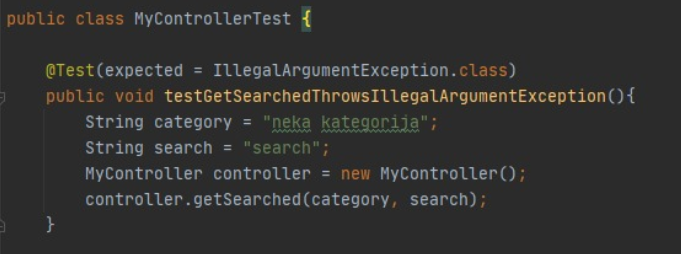
\includegraphics[scale=1]{dokumentacija/slike/testSearch.PNG} %veličina slike u odnosu na originalnu datoteku i pozicija slike
            \centering
            \label{fig:promjene}
            \end{figure}
			
			Rezultat izvođenja testa jest javljanje IllegalArgumentException, te su uvjeti testa zadovoljeni, i aplikacija je prošla test.
			
		\pagebreak
			
		\textbf{Ispitni slučaj 2: testiranje funkcionalnosti metode validateEmail() }
			
			Cilj ovog testa jest provjeriti rad funkcije testEmailValidation na način da se za 2 String vrijednosti (od kojih je jedna ispravna a druga neispravna) pozove dotična metoda.
		    \vspace{3mm} %3mm vertical space
		    
			Ulaz:
			\begin{packed_enum}
			    \item String koji predstavlja email korisnika
			\end{packed_enum}
			
			\text{Očekivani rezultat:}
			\noindent
			\begin{packed_enum}
			    \item za ispravan format email adrese vraća true
			    \item za neispravan format email adrese vraća false

			\end{packed_enum}
			
			\begin{figure}[H]
            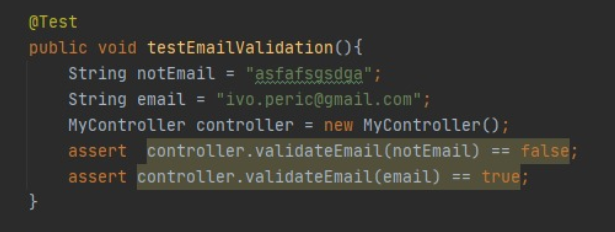
\includegraphics[scale=1]{dokumentacija/slike/testMail.PNG} %veličina slike u odnosu na originalnu datoteku i pozicija slike
            \centering
            \label{fig:promjene}
            \end{figure}
			
			Rezultat izvođenja testa je odgovarajuć, te su uvjeti testa zadovoljeni, i aplikacija je prošla test.
		
		  \vspace{10mm} %10mm vertical space
		
		\textbf{Ispitni slučaj 3: testiranje funkcionalnosti metode getHash() }
			
		Rad metode testHashingFunction provjeravamo na način da kao ulaz u funkciju pripremimo proizvoljan String tekst, za koji unaprijed znamo koji mu je hash kod. Pozivom naše funkcije, promatramo rezultat.
		\vspace{3mm} %3mm vertical space

		Ulaz:
		\noindent
		\begin{packed_enum}
		    \item String koji predstavlja String tekst za koji provjeravamo hash kod.
		    \item String vrijednost unaprijed izračunatog hash koda.
		\end{packed_enum}
		
		\text{Očekivani rezultat:}
		\noindent
		\begin{packed_enum}
		    \item usporedba unaprijed izračunate hash vrijednosti i rezultata funkcije je jednaka

		\end{packed_enum}
		
		\begin{figure}[H]
            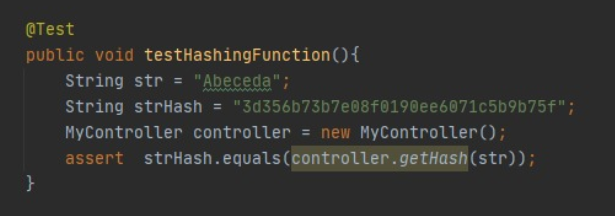
\includegraphics[scale=1]{dokumentacija/slike/testHash1.PNG} %veličina slike u odnosu na originalnu datoteku i pozicija slike
            \centering
            \label{fig:promjene}
            \end{figure}
			
		Rezultat izvođenja testa je odgovarajuć, te su uvjeti testa zadovoljeni, i aplikacija je prošla test.
		
		\vspace{10mm} %10mm vertical space
		
		\textbf{Ispitni slučaj 4: testiranje dodatne funkcionalnosti metode getHash() }
			
		Rad metode testHashingFunction dodatno ćemo provjeriti tako što ćemo ponoviti postupak kao u prethodnom testu, samo što ćemo umjesto ispravne vrijednosti unaprijed izračunate hash vrijednosti, koristiti neispravnu vrijednost.
		\vspace{3mm} %3mm vertical space
		
		Ulaz:
		\noindent
		\begin{packed_enum}
		    \item String koji predstavlja String tekst za koji provjeravamo hash kod.
		    \item String vrijednost unaprijed izračunatog krivog hash koda.
		\end{packed_enum}
		
		\text{Očekivani rezultat:}
		\noindent
		\begin{packed_enum}
		    \item usporedba unaprijed izračunate hash vrijednosti i rezultata funkcije je različita

		\end{packed_enum}
		
		\begin{figure}[H]
            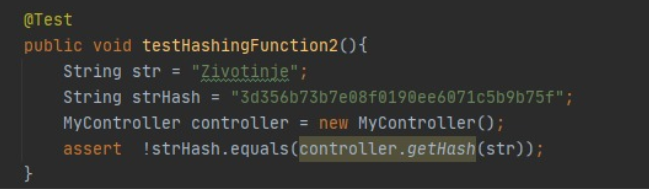
\includegraphics[scale=1]{dokumentacija/slike/testHash2.PNG} %veličina slike u odnosu na originalnu datoteku i pozicija slike
            \centering
            \label{fig:promjene}
            \end{figure}
			
		Rezultat izvođenja testa je odgovarajuć, te su uvjeti testa zadovoljeni, i aplikacija je prošla test.
		
        
        \pagebreak
        
		\textbf{Ispitni slučaj 5: testiranje funkcionalnosti dodavanja aktivnosti u raspored}
			
		Cilj ovog testa jest provjeriti ispravnost rada funkcije testActivityComparator. Konkretnije, ispitujemo je li redosljed aktivnosti u rasporedu ispravan.
		
		\vspace{3mm} %10mm vertical space
		Ulaz:
		\noindent
		\begin{packed_enum}
		    \item Aktivnost u vremenu koja počinje 15.5.2020.
		    \item Aktivnost u vremenu koja počinje 1.1.2021.
		\end{packed_enum}
		
		\text{Očekivani rezultat:}
		\noindent
		\begin{packed_enum}
		    \item U prvom slučaju, pozivom metode after(), koja utvrđuje je li prva aktivnost nakon druge u rasporedu aktivnosti, rezultat očekujemo da bude false
		    
		    \item U drugom slučaju, zamijenimo uloge aktivnosti te očekujemo rezultat true.

		\end{packed_enum}
		
		\begin{figure}[H]
            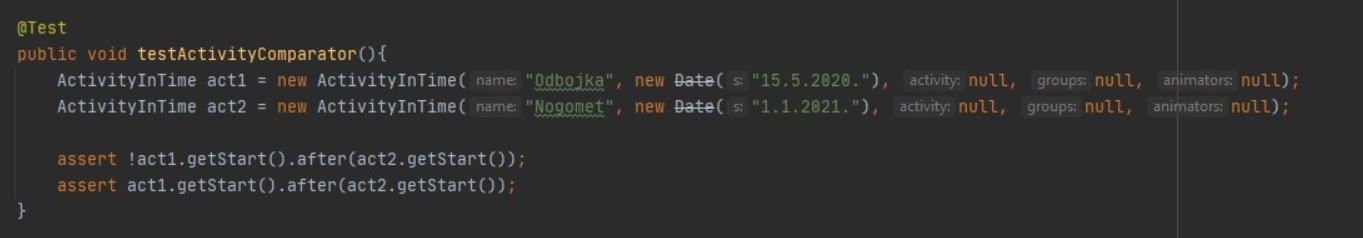
\includegraphics[width=15cm]{dokumentacija/slike/testRaspored.PNG} %veličina slike u odnosu na originalnu datoteku i pozicija slike
            \centering
            \label{fig:promjene}
            \end{figure}
			
		Rezultat izvođenja testa je odgovarajuć, te su uvjeti testa zadovoljeni, i aplikacija je prošla test.
		
		\vspace{10mm} %10mm vertical space
		
		\textbf{Ispitni slučaj 6: testiranje funkcionalnosti metode validateNumberOfGroups() }
			
		Cilj ovog testa jest provjeriti ispravnost rada funkcije testActivityComparator. Konkretnije, ispitujemo hoće li aplikacija baciti grešku ako kao tip aktivnosti pošaljemo neispravnu vrijednost.
		
		\vspace{3mm} %10mm vertical space
		Ulaz:
		\noindent
		\begin{packed_enum}
		    \item Aktivnost s neispravno postavljenim tipom aktivnosti
		\end{packed_enum}
		
		\text{Očekivani rezultat:}
		\noindent
		\begin{packed_enum}
		    \item Pozivom metode, aplikacija treba baciti IllegalArgumentException

		\end{packed_enum}
		
		\begin{figure}[H]
            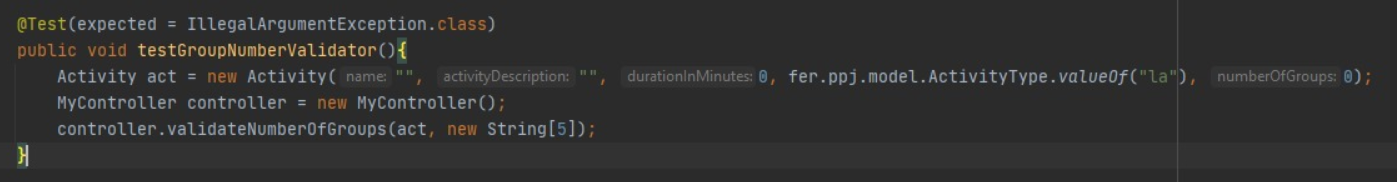
\includegraphics[width=15cm]{dokumentacija/slike/testGrupa.PNG} %veličina slike u odnosu na originalnu datoteku i pozicija slike
            \centering
            \label{fig:promjene}
            \end{figure}
			
		Rezultat izvođenja testa je odgovarajuć, te su uvjeti testa zadovoljeni, i aplikacija je prošla test.
		
		\pagebreak
			
			
			\subsection{Ispitivanje sustava}
			
			Svi testovi izvršeni su pomoću Selenium IDE-a. Ispitivanje sustava je provedeno po obrascima uporabe kako bi se provjerila osnova funkcionalnost sutava, ali i nasumičnim kretanjima po aplikaciji kako bi se pronašle neočekivane greške ili nepredviđena ponašanja. Prikazivanje ispitivanja UC2, UC3, UC 13, UC 15.
			
			\textbf{}
			
			\textbf{Ispitni slučaj 1: Registracija}
			
			\textbf{Ulaz:}
			\begin{enumerate}
			    \item Korisnik odabire opciju registracije
			    \item Korisnik unosi potrebne korisničke podatke
			    \item Korisnik prima email o uspješnoj registraciji i odabire šifru za svoj račun u sustvavu
			\end{enumerate}
			
			\textbf{Očekivani rezultat:}
			
			\begin{enumerate}
			    \item Korisnik je primio email i registrirao se
			\end{enumerate}
			
			\textbf{Rezultat:} 
			
			\begin{figure}[H]
            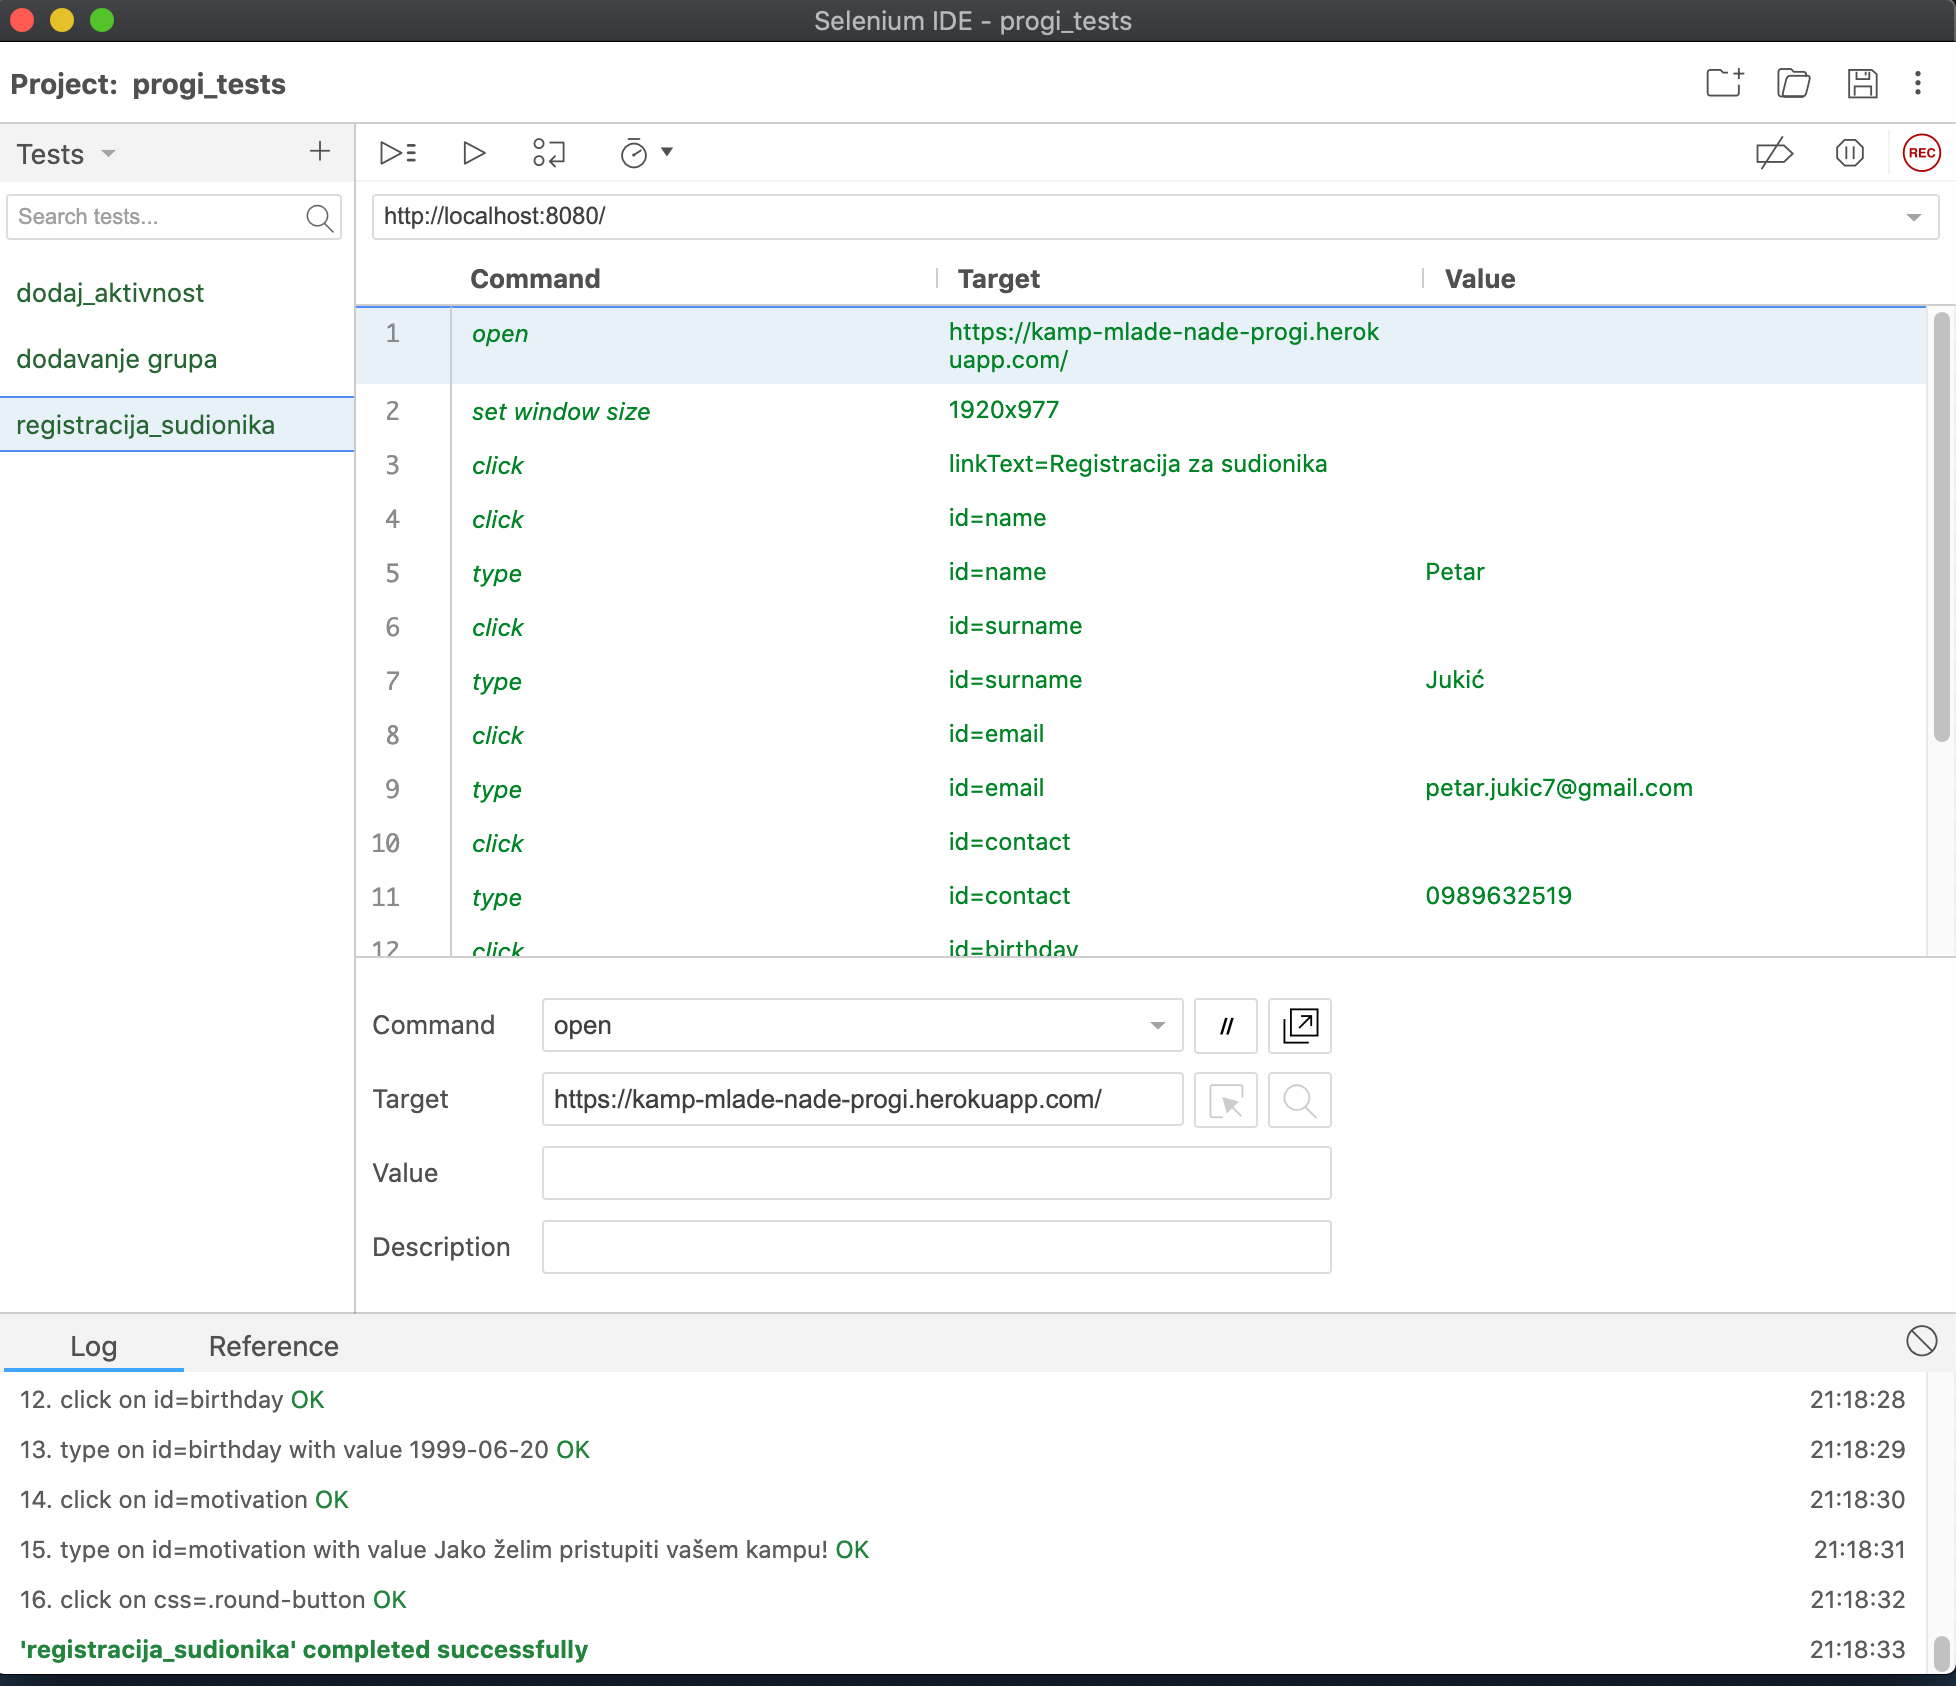
\includegraphics[scale=0.378]{dokumentacija/slike/REGISTRACIJA_TEST.png} %veličina slike u odnosu na originalnu datoteku i pozicija slike
            \centering
            \textbf{}
            
            Korisnik je uspješno registriran i primio je mail.
            \label{fig:promjene}
            \end{figure}
            
            \begin{figure}[H]
            
\includegraphics[scale=0.5]{dokumentacija/slike/MAIL_PRIMLJEN_U_KAMP.png} %veličina slike u odnosu na originalnu datoteku i pozicija slike
            \centering
            Korisnik primi mail ako je uspješno registriran.
            \label{fig:promjene}
            \end{figure}
			
			\textbf{}
			\textbf{}
			\textbf{Ispitni slučaj 2: Prijava u sustav (prije početka kampa) - sudionici}
			
			\textbf{Ulaz:}
			\begin{enumerate}
			    \item Unos korisničkog imena i lozinke
			    \item Potvrda o ispravnosti unesenih podataka
			\end{enumerate}
			
			\textbf{Očekivani rezultat:}
			
			\begin{enumerate}
			    \item Korisniku se prikazuje sat koji odbrojava do početka kampa.
			\end{enumerate}
			
			\textbf{Rezultat:} 
			
			\begin{figure}[H]
            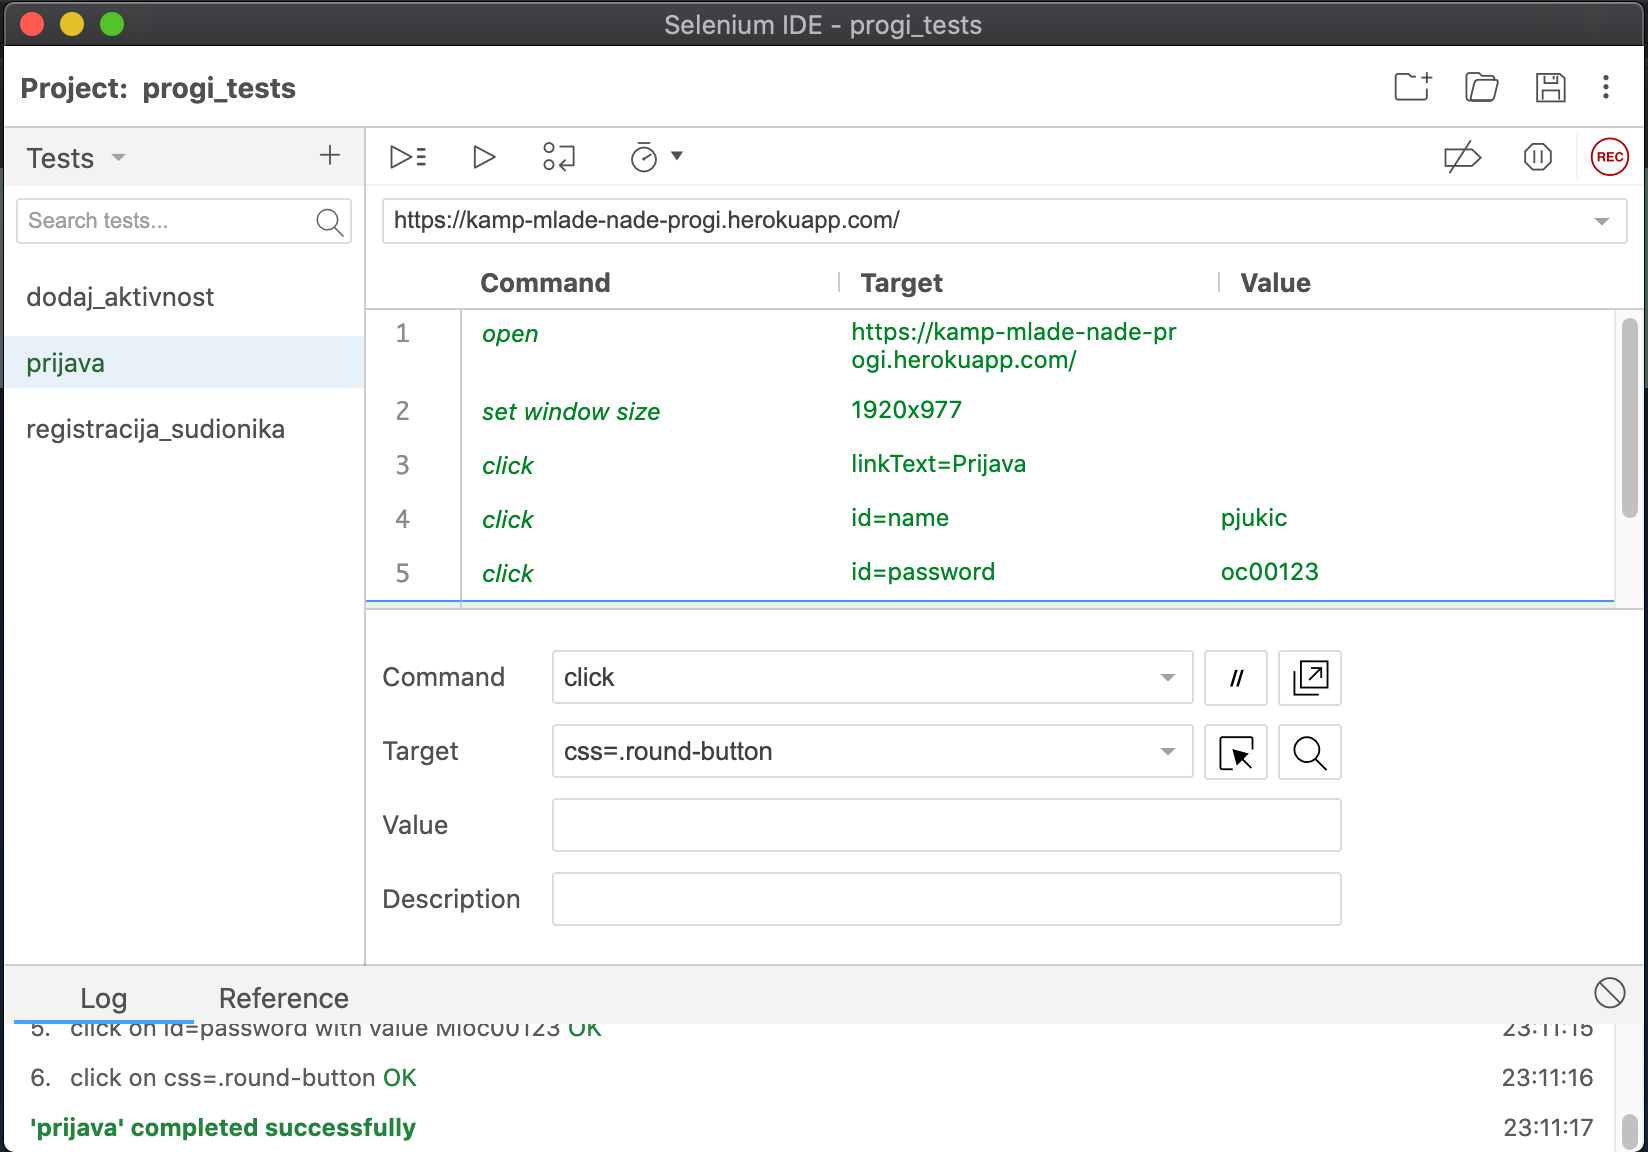
\includegraphics[scale=0.5]{dokumentacija/slike/PRIJAVA_SUDIONIKA.png} %veličina slike u odnosu na originalnu datoteku i pozicija slike
            \centering
            Test je prošao.
            \label{fig:promjene}
            \end{figure}
            
            \begin{figure}[H]
            
\includegraphics[scale=0.43]{dokumentacija/slike/ODBROJAVANJE_SAT_23.26.10.png} %veličina slike u odnosu na originalnu datoteku i pozicija slike
            \centering
            Odbrojavanje sata.
            \label{fig:promjene}
            \end{figure}
			
			\textbf{}
			
			\textbf{Ispitni slučaj 3: Definiranje aktivnosti}
			
			\textbf{Ulaz:}
			\begin{enumerate}
			    \item Organizator unosi podatke za definiranje nove aktivnosti (ime, kratki opis, vremensko trajanje, tip aktivnosti)
			\end{enumerate}
			
			\textbf{Očekivani rezultat:}
			
			\begin{enumerate}
			    \item Stvorena je nova aktivnost
			\end{enumerate}
			
			\textbf{Rezultat:} 
			
			\begin{figure}[H]
            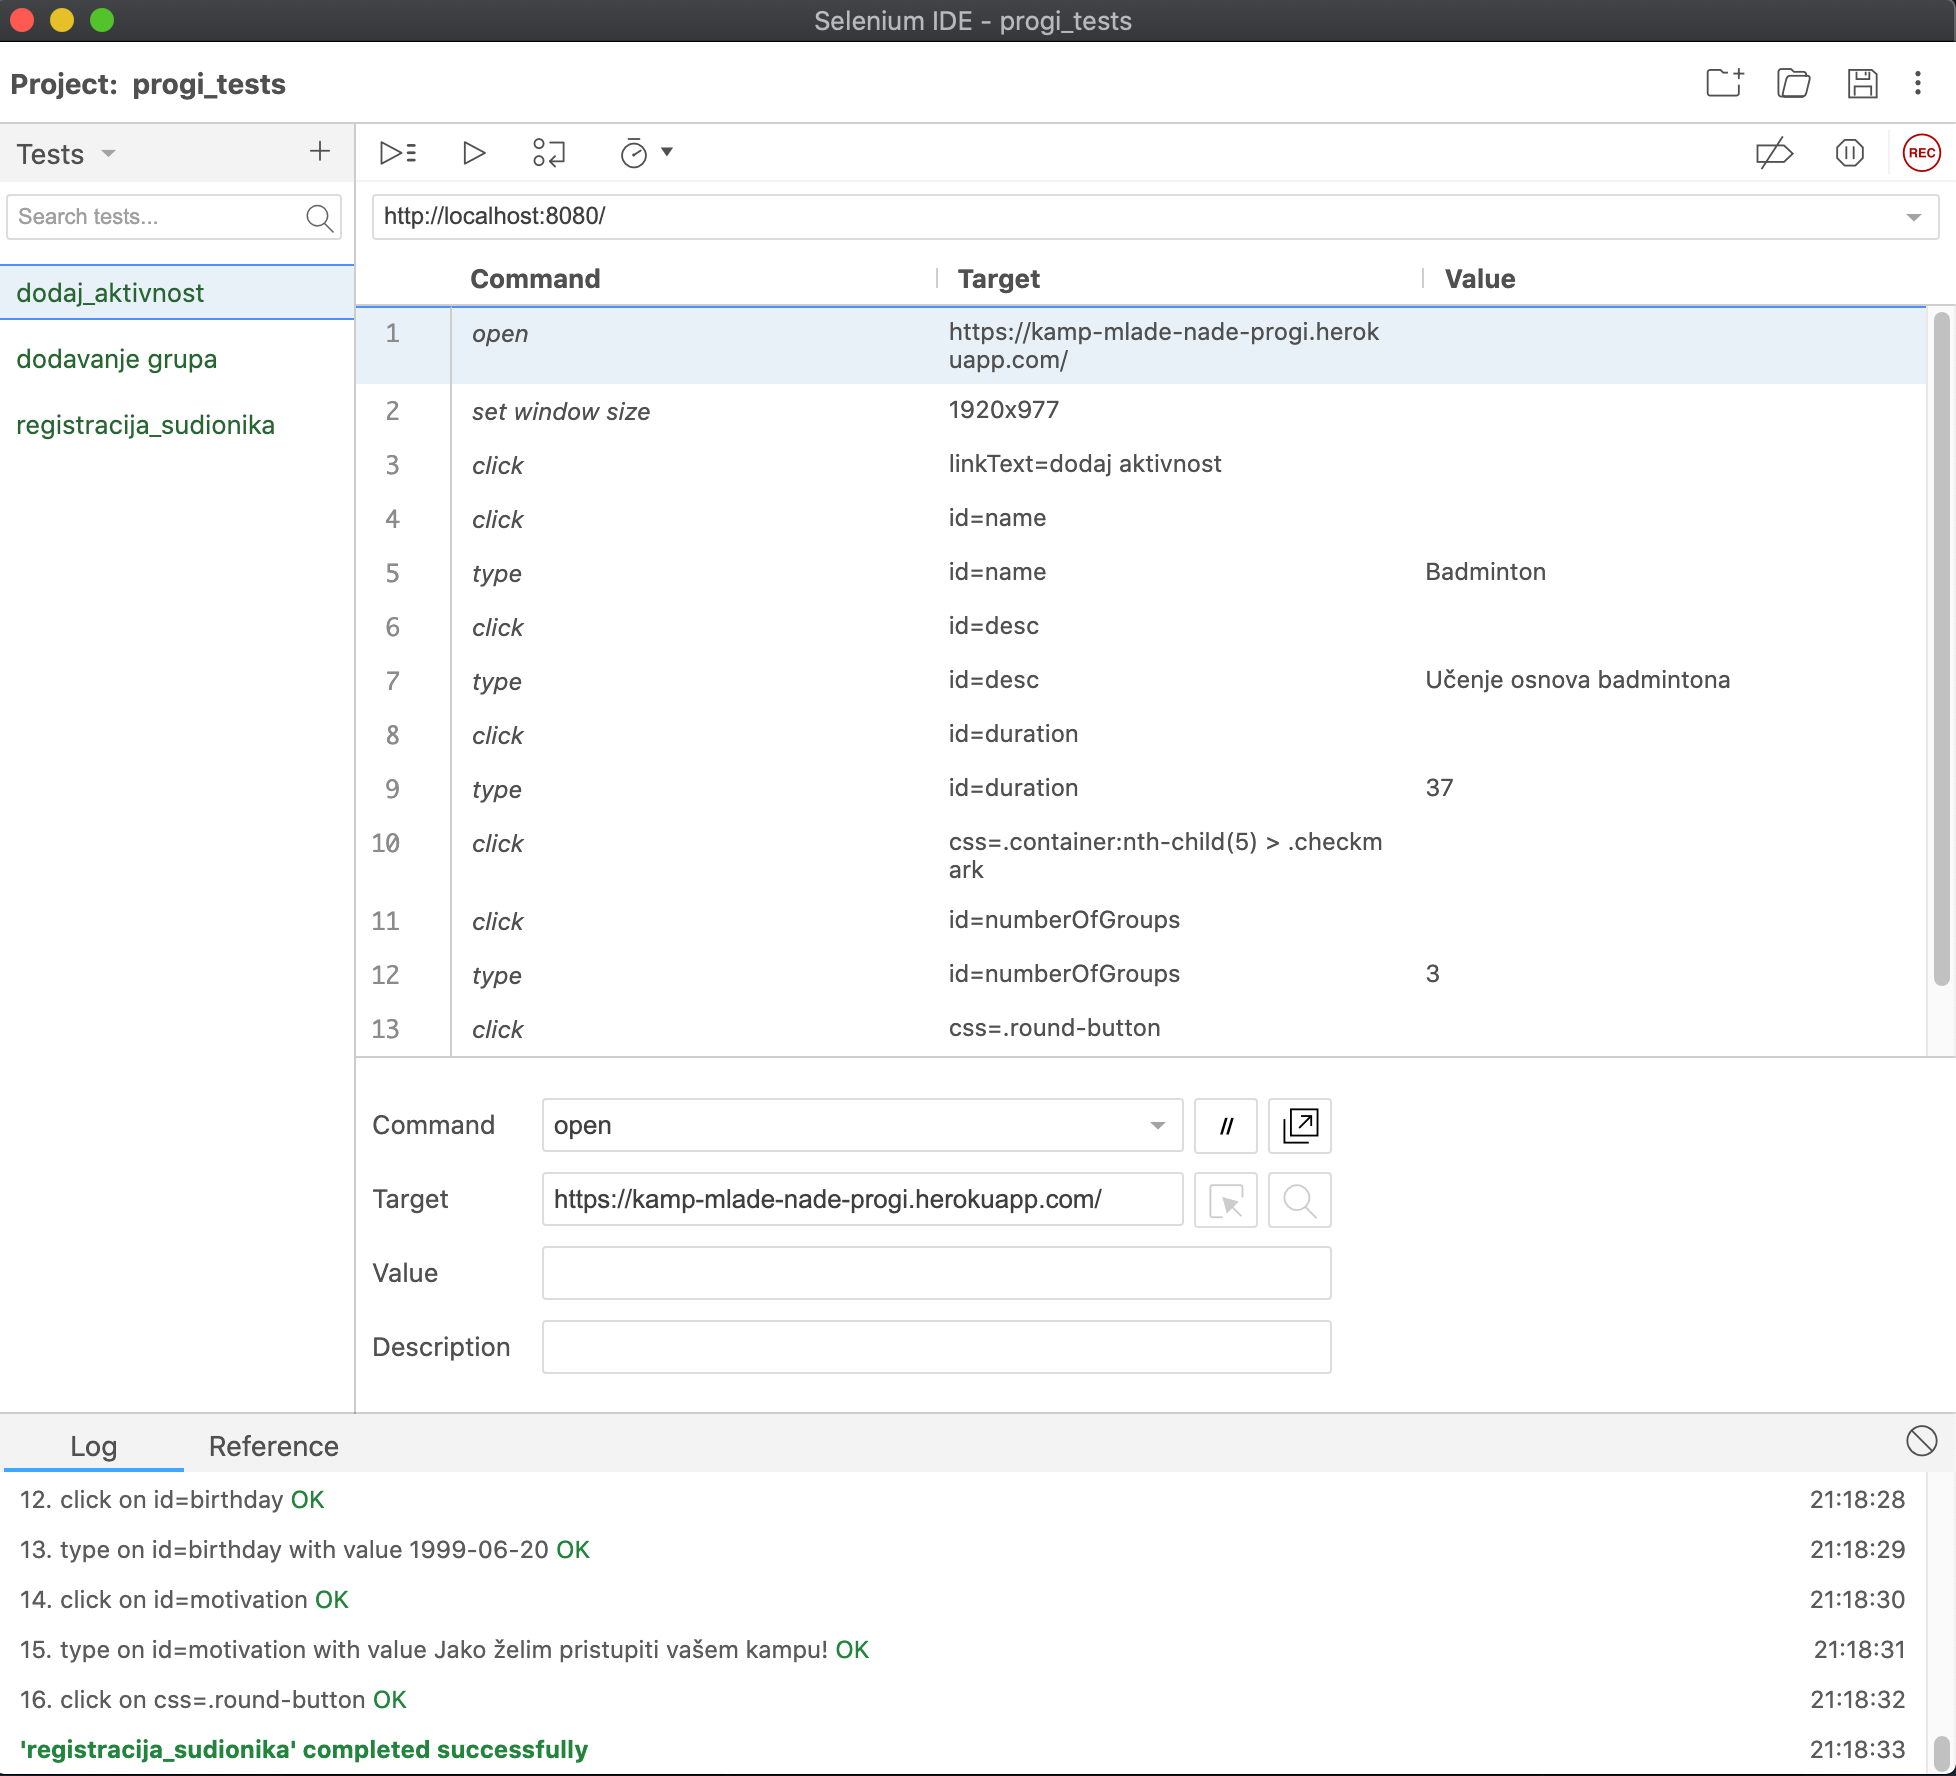
\includegraphics[scale=0.3]{dokumentacija/slike/DODAJ_AKTIVNOSTI_TEST.png} %veličina slike u odnosu na originalnu datoteku i pozicija slike
            \centering
            
            Test je prošao.
            \label{fig:promjene}
            \end{figure}
    
            \begin{figure}[H]
            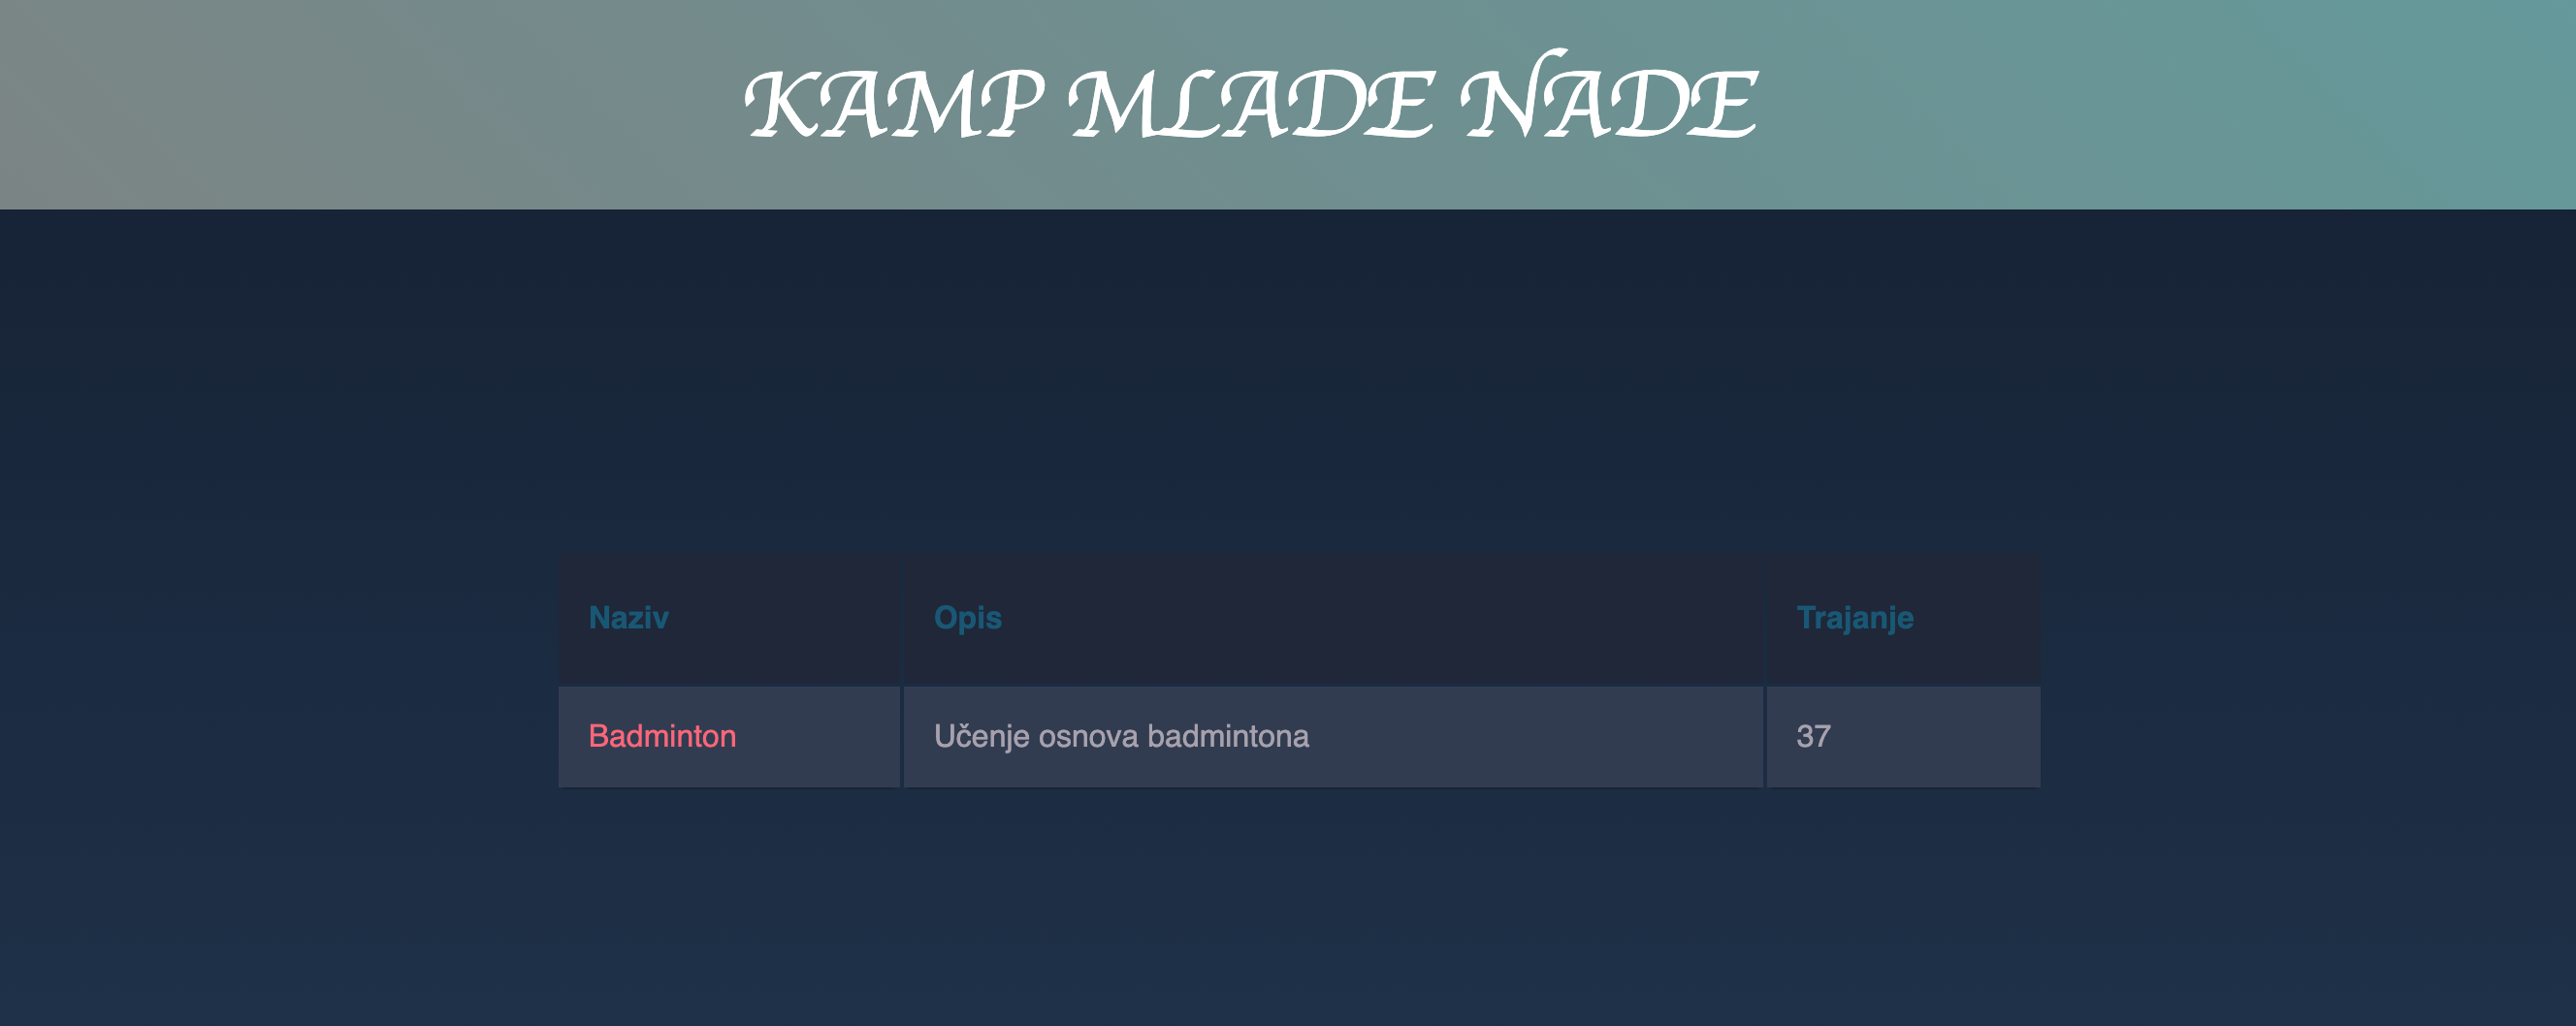
\includegraphics[scale=0.35]{dokumentacija/slike/DODAVANJE_AKTIVNOSTI.png} %veličina slike u odnosu na originalnu datoteku i pozicija slike
            \centering
            Aktivnost je dodana.
            \label{fig:promjene}
            \end{figure}
			
			\textbf{}
			\newline
			
			
			\textbf{Ispitni slučaj 4: Određivanje broja grupa}
			
			\textbf{Ulaz:}
			\begin{enumerate}
			    \item Organizator vidi popis svih uspješno prijavljenih sudionika i odabire željeni broj grupa u brojčanom obliku
			\end{enumerate}
			
			\textbf{Očekivani rezultat:}
			
			\begin{enumerate}
			    \item Izvršava se automatska dodjela sudionika u grupe
			\end{enumerate}
			\pagebreak
			\textbf{Rezultat:} 
			\begin{figure}[H]
            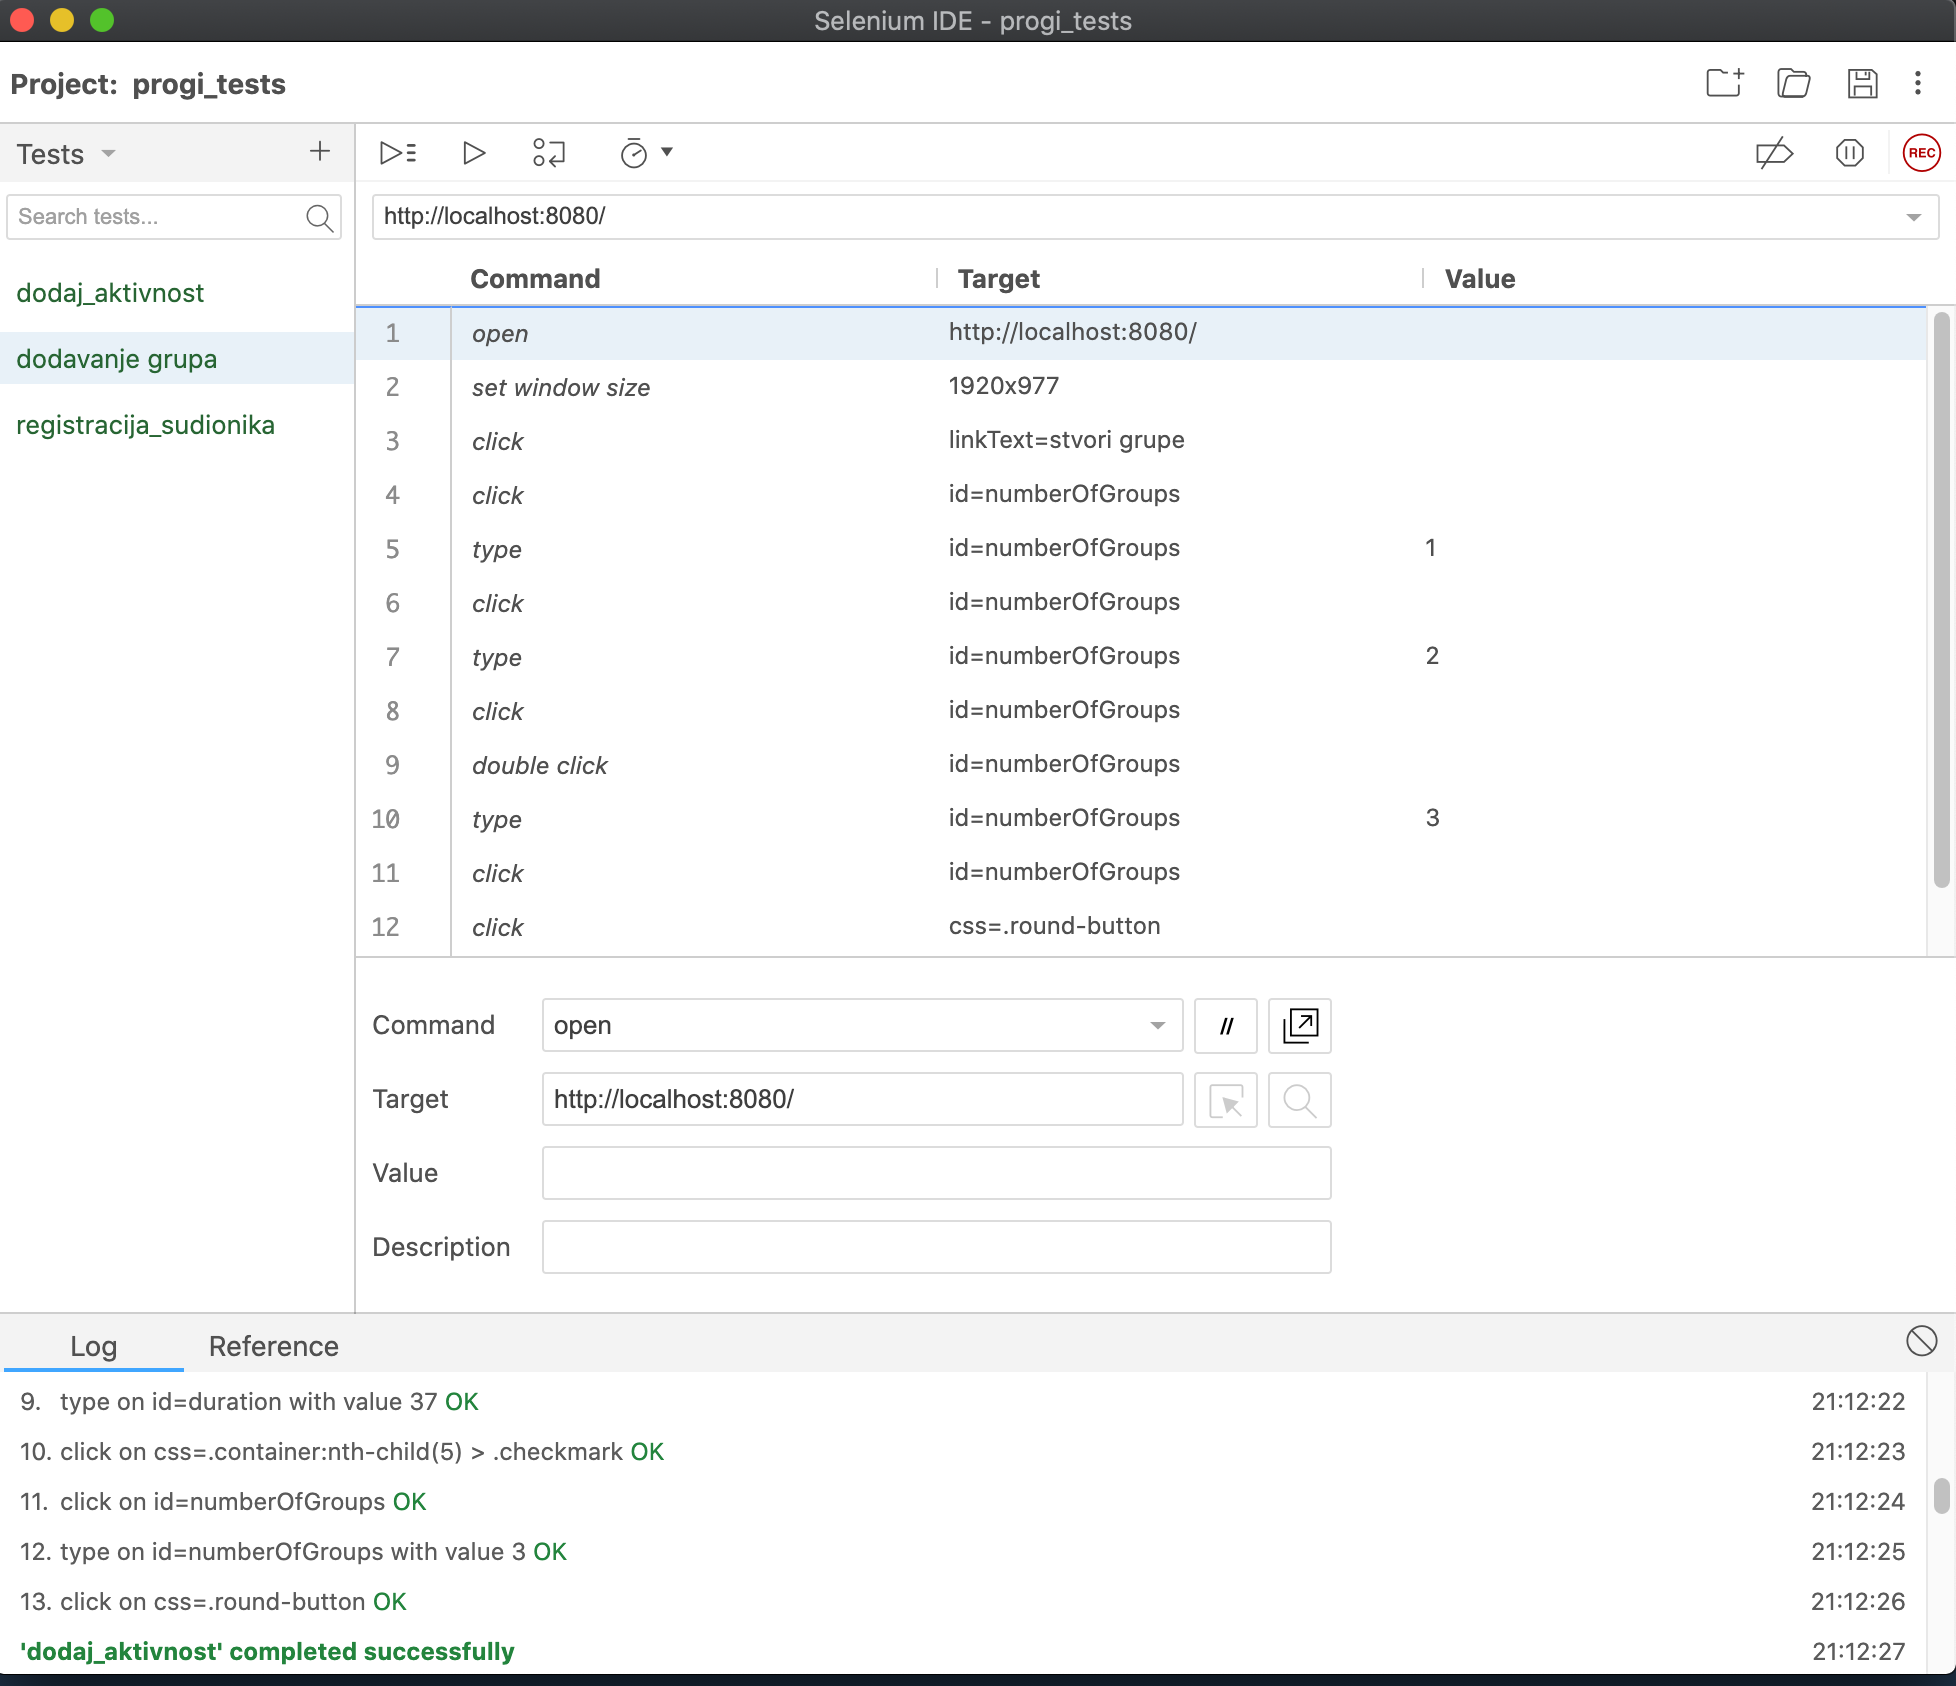
\includegraphics[scale=0.45]{dokumentacija/slike/DODAVANJE_GRUPA_TEST.png} %veličina slike u odnosu na originalnu datoteku i pozicija slike
            \centering
            Test je prošao i dodane su grupe.
            \label{fig:promjene}
            \end{figure}			
			\eject 
		
		
		
		\section{Dijagram razmještaja}
			
        Dijagrami razmještaja opisuju topologiju programske potpore kako bi elementi sustava bili optimalno raspoređeni. Sustav je baziran na "klijent-poslužitelj" arhitekturi. Korisnička računala razmjenjuju podatke sa centraliziranim serverom, a Server sadrži sve potrebne datoteke i aplikacije koje šalje korisnicima na zahtjev. Komunikacija između korisnika i poslužitelja odvija se preko HTTPS veze.
		\newline
		\newline
		\newline
		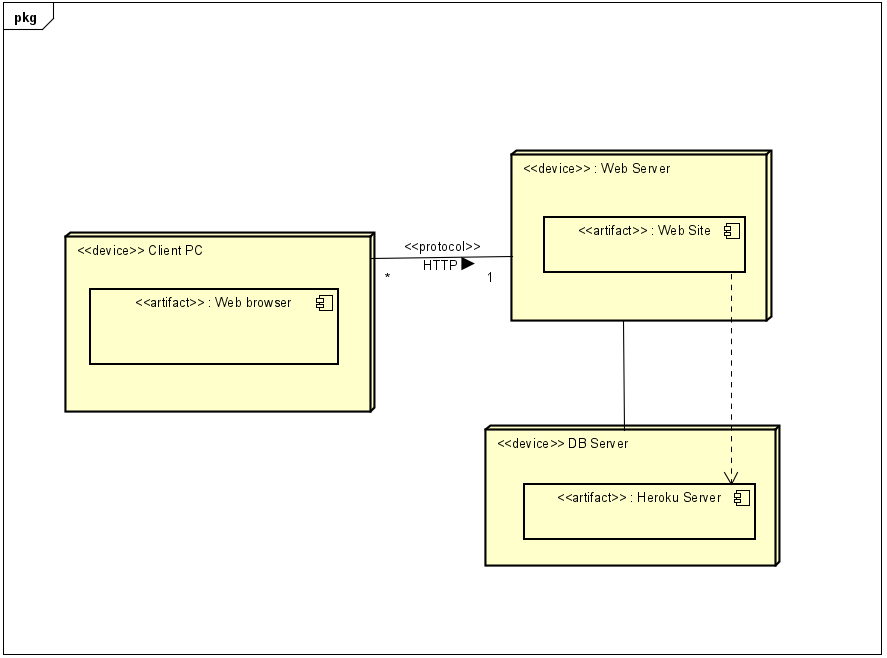
\includegraphics[scale=0.85]{slike/dijagramRazmjestaja.png}
			
			\eject 
		
		\section{Upute za puštanje u pogon}
		
		    \textbf{Instalacija PostgreSQL sustava za upravljanje bazom podataka}
		    
		    Potrebno je preuzeti instalacijski program sa sljedeće poveznice \url{https://www.postgresql.org/download/}. Odabrati odgovarajući operacijski sustav i pritisnuti \textit{Download installer}.
		    
		        \textbf{Konfiguracija i instalacija}
		        \begin{enumerate}
		            \item Pokrenuti instalacijski program te zatim čarobnjak za konfiguraciju instalacije
		            \item Za direktorij je preporučeno ostaviti predloženu putanju
		            \item Kod odabira kompopnenti sustava koje će biti instalirane obavezno označiti komponente : \textbf{PosgreSQL} Server i \textbf{PgAdmin4}
		            \item Kod odabira direktorija za pohranu podataka, preporuka je ostaviti predloženu putanju
		            \item Unijeti lozinku za admin korisnika
		            \item Ostaviti predložena vrata (port) za pristup sustavu baze podataka : 5432
		            \item Odabrati lokalne postavke
		            \item Kliknuti Next, pričekati završetak instalacije te zatim kliknuti Finsih
		        \end{enumerate}
		        
		        \textbf{Kreiranje baze podataka}
		        
		        Za interakciju s poslužiteljem PostgreSQL koristit ćemo \textit{pgAdmin} program. Prvi prvom pokretanju traži da postavite "master" lozinku - upišite onu koju ste postavili u gornjim koracima. Nakon unosa lozinke otvoriti u prozoru "Browser" listu "Servers" i kliknite na znak strijelice pored "PostgreSql 12". Ponovo unesite lozinku za korisnika postgres. 
		        Odabirom "Databases" u prozoru "Browser" desnim klikom odabrati "Create - Database". Unijeti ime baze podataka \textit{projekt} i kliknuti na gumb Save.
		        \newline 
		        
		\noindent \textbf{Instalacija alata Apache Maven}
		
		Za potrebe pokretanja naše aplikacije bitna stavka je instalacija alata Maven. 
		
		\begin{itemize}
		    \item Sa stranice \url{https://maven.apache.org/download.cgi} skinuti distribuciju arhive u tar.gz ili zip formatu
		    \item Provjeriti da je JAVA HOME varijabla pravilno podešena
		    \item Ekstratirati distribuciju arhive na željenu lokaciju
		    \item Dodati bin direktorij novostvorenog direktorija apache-maven-3.6.3 u PATH varijablu
		    \item Provjeriti sa mvn -v uspješnost instalacije.  
		\end{itemize}
			
		\noindent \textbf{Konfiguracija veze s bazom podataka}
		
		Da bi aplikacija uspješno koristila bazu podataka, potrebno je postaviti parametre konekcije s bazom podataka u datoteci \textbf{application.properties} u direktoriju \textbf{resources}. Potrebno je izmijeniti sljedeće linije:
		\newline
		spring.datasource.username=postgres
		\newline
        spring.datasource.password=\textit{upisati lozinku odabranu u prethodnim koracima}
        \newline
        spring.datasource.url=jdbc:postgresql://localhost:5432/projekt

        \newline
        \newline
        \textbf{}
		
		\noindent \textbf{Pokretanje web aplikacije}
			
			U terminalu se pozicionirati unutar vršnog direktorija u kojem je projekt. Pokrenuti naredbu mvn spring-boot:run.
			
			Web aplikacija je sada dostupna na adresi \url{http://localhost:8080/}
			
			
			
	
			\eject 
